\documentclass[../main.tex]{subfiles}
\graphicspath{{\subfix{../Images/}}}
\begin{document}

\section{Model Performance} \label{performance}


%%%%%%%%%%%%%%%%%%%%%%%%%%%%%%%%%%%%%%%%%%%%%%%%%%%%%%%%%%%%%%%%%%%%
%\subsection{Yolo Performance} \label{yolo_performance}

%%%%%%%%%%%%%%%%%%%%%%%%%%%%%%%%%%%%%%%%%%%%%%%%%%%%%%%%%%%%%%%%%%%%
% \subsection{Transfer Learning and Model Fine-Tuning}
% \label{sec:yolo_finetuning}
% For this research, YOLOv8 was trained on a custom maritime dataset derived from sensor recordings collected aboard the Minion platform.
% The dataset includes labeled examples of navigation markers, buoys, vessels, and other relevant maritime objects captured under diverse lighting conditions, sea states, and viewing angles.
% Transfer learning was employed by initializing the network with weights pre-trained on a general-purpose dataset, then fine-tuning on the maritime-specific data to adapt the model to the target domain.

% Inference was conducted using the YOLOv8m variant, selected to balance detection accuracy with real-time performance on the GPU-equipped computing platform installed on Minion.
% Post-processing applies non-maximum suppression to eliminate redundant detections, retaining only the highest-confidence predictions for each detected object.
% Pre-trained YOLOv8 weights were fine-tuned on a domain-specific dataset collected from the Minion \ac{ASV} platform.  
% Transfer learning accelerates convergence and reduces the need for large labeled datasets by adapting weights from a general-purpose model (e.g., COCO) to the maritime environment.

% Fine-tuning was performed using the Ultralytics YOLOv8 framework \cite{ultralytics}, with a combination of data augmentation techniques (random flips, exposure shifts, and rotations) to increase robustness under variable lighting and sea-state conditions.
% Hyperparameters such as learning rate, batch size, and number of epochs were optimized empirically to prevent overfitting while ensuring consistent convergence.

% % \begin{figure}[htbp]
% %     \centering
% %     \includegraphics[width=0.85\linewidth]{Images/yolo_training_curve.png}
% %     \caption{Example YOLOv8 training convergence showing loss and mean Average Precision (mAP) trends over epochs.}
% %     \label{fig:yolo_training_curve}
% % \end{figure}


% To assess the tradeoff between accuracy and inference speed, three YOLOv8 variants—\textit{nano/xs}, \textit{small}, and \textit{medium}—were evaluated.
% Each model differs in backbone depth and channel width, providing progressively higher accuracy at the cost of computational complexity.
% % Table~\ref{tab:yolo_variants} summarizes model specifications and benchmark performance.

% % \begin{table}[htbp]
% % \centering
% % \caption{YOLOv8 model comparison for visual detection tasks.}
% % \begin{tabularx}{0.9\textwidth}{l c c c c}
% % \toprule
% % \textbf{Model} & \textbf{Params (M)} & \textbf{Input Size (px)} & \textbf{FPS (RTX 3090)} & \textbf{mAP@50} \\
% % \midrule
% % YOLOv8-xs & 3.2 & 640 & 110 & 0.79 \\
% % YOLOv8-s & 11.2 & 640 & 85 & 0.84 \\
% % YOLOv8-m & 25.9 & 640 & 63 & 0.87 \\
% % \bottomrule
% % \end{tabularx}
% % \label{tab:yolo_variants}
% % \end{table}

% Inference timing was recorded using per-process timers to isolate image capture, pre-processing, neural inference, and post-processing durations.
% This timing-based comparison allows fair assessment against non-GPU LiDAR pipelines in later sections.

% %%%%%%%%%%%%%%%%%%%%%%%%%%%%%%%%%%%%%%%%%%%%%%%%%%%%%%%%%%%%%%%%%%%%
% \subsection{Retraining Results and Performance Evaluation}
% \label{sec:yolo_results}

% The fine-tuned YOLOv8-s model achieved the best balance of accuracy and speed for maritime operations.
% Model evaluation was performed using a holdout dataset collected under variable illumination and sea states.
% Performance metrics include mean Average Precision (mAP@50), precision-recall curves, and confusion matrices for key object classes such as vessels, buoys, and docks.

% \begin{figure}[htbp]
%     \centering
%     \includegraphics[width=0.8\linewidth]{Images/yolo_confusion_matrix.png}
%     \caption{Confusion matrix for YOLOv8-s model evaluated on the test dataset.}
%     \label{fig:yolo_confusion_matrix}
% \end{figure}

% \begin{figure}[htbp]
%     \centering
%     \includegraphics[width=0.8\linewidth]{Images/yolo_pr_curve.png}
%     \caption{Precision–recall curve for primary object classes.}
%     \label{fig:yolo_pr_curve}
% \end{figure}

% Results indicate consistent detection performance across lighting conditions with minimal false positives on horizon clutter.
% Retraining improved small-object detection by approximately X\% compared to baseline COCO-trained weights, confirming the benefit of domain adaptation for maritime imagery.

% %%%%%%%%%%%%%%%%%%%%%%%%%%%%%%%%%%%%%%%%%%%%%%%%%%%%%%%%%%%%%%%%%%%%
% \subsection{Discussion and Relevance to Sensor Fusion}
% \label{sec:yolo_discussion}

% The fine-tuned YOLOv8 network serves as the visual baseline for comparison with LiDAR-based object detection methods presented in Section~\ref{gbcache}.
% By isolating timing metrics for each processing stage, the performance comparison remains hardware-agnostic.
% This approach emphasizes algorithmic latency, rather than total frame rate, as the primary metric for evaluating real-time feasibility in multi-sensor fusion.

%%%%%%%%%%%%%%%%%%%%%%%%%%%%%%%%%%%%%%%%%%%%%%%%%%%%%%%%%%%%%%%%%%%%
\subsection{Computational Efficiency} \label{sec:gbcache_efficiency}

The algorithmic design of \ac{GB-CACHE} prioritizes computational efficiency to enable real-time processing on autonomous surface vessel hardware with limited computing resources.
Grid-based spatial indexing reduces clustering complexity from quadratic to linear in the number of points, while the regular grid structure enables vectorized operations and cache-efficient memory access patterns.
These optimizations prove essential for maintaining detection frame rates sufficient for autonomous navigation, where delayed perception degrades collision avoidance performance.

The GB-CACHE processing pipeline operates incrementally on each \ac{LiDAR} scan, maintaining no temporal history and requiring no iterative refinement.
This design guarantees bounded worst-case execution time, critical properties for safety-critical autonomous systems.
Each scan undergoes independent processing: grid population, clustering, hull extraction, and feature calculation, producing object detections with consistent latency.

Memory requirements scale with grid dimensions rather than point count, providing predictable resource consumption independent of scene complexity.
The grid representation compresses sparse maritime point clouds into compact occupancy structures, reducing memory bandwidth requirements compared to maintaining full point coordinates.
This compression proves particularly advantageous for maritime environments where objects occupy a small fraction of the sensor's field of view.

\begin{figure}
    \centering
    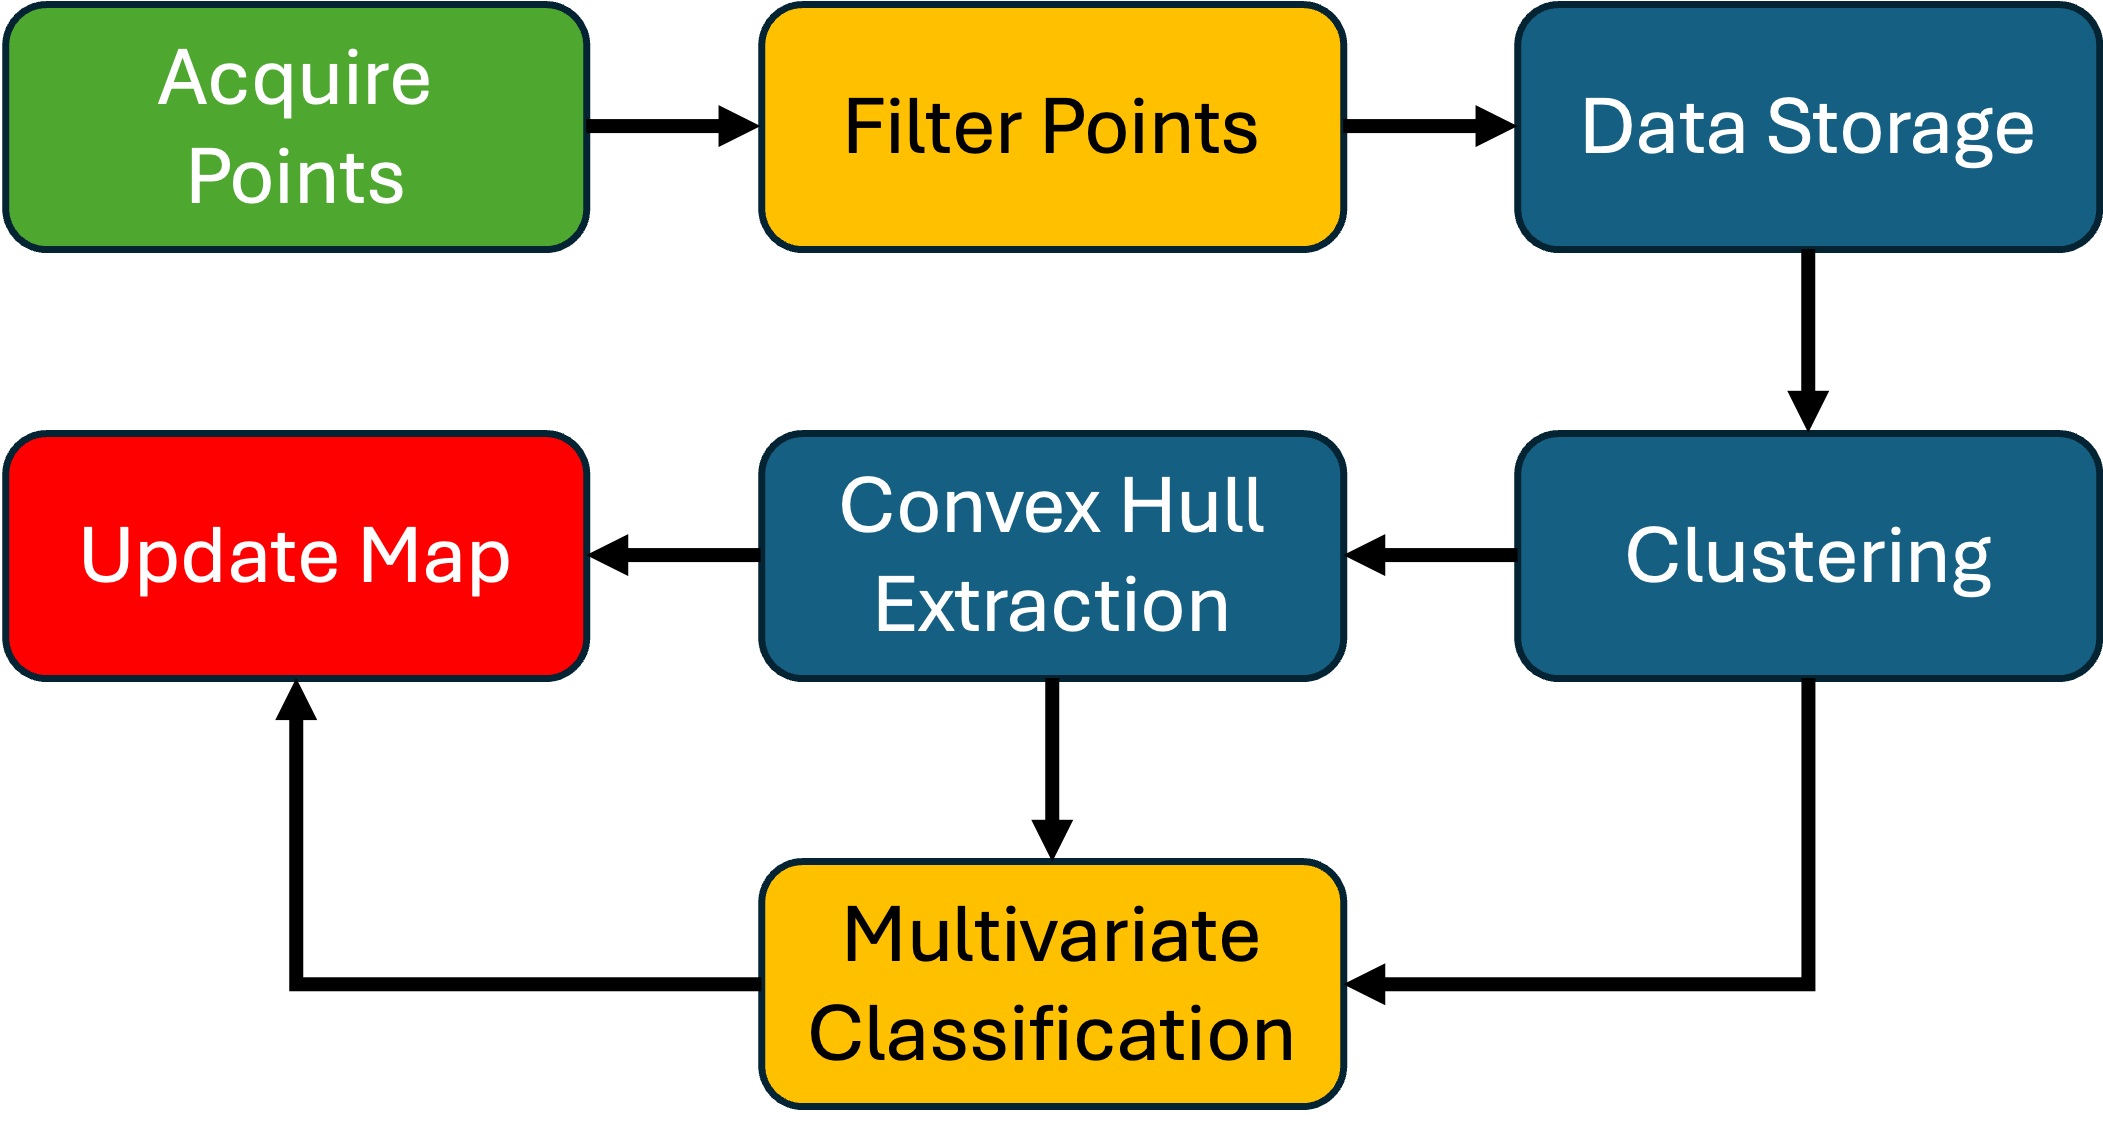
\includegraphics[width=0.95\linewidth]{Images/gbcache_flow.png}
    \caption{Caption}
    \label{fig:gbcache_flow}
\end{figure}

Performance analysis of the \ac{GB-CACHE} implementation on the Minion platform demonstrates exceptional computational efficiency compatible with real-time autonomous navigation requirements.
The spatial filtering and point addition operations execute with sub-millisecond latency, consuming negligible fractions of available processing time at sensor frame rates.
The map update operation, while more computationally intensive, exhibits strong linear correlation with object geometric complexity, specifically polygon perimeter and surface area.
This predictable scaling behavior enables reliable worst-case execution time estimation for safety-critical autonomous systems.
Hardware resource utilization remains minimal during typical operation, with both processor and memory consumption well below capacity thresholds, providing substantial computational headroom for concurrent navigation and control processes.
Detailed performance characterization across diverse maritime object encounters validates the algorithm's suitability for sustained real-time operation under operational constraints.

\begin{figure}[htbp]
\centering
\makebox[\textwidth][c]{
    \begin{subfigure}[t]{0.44\textwidth}
        \centering
        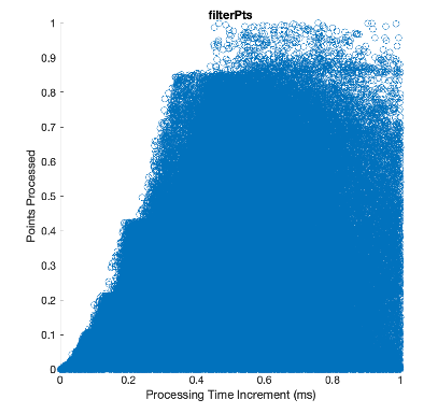
\includegraphics[width=\textwidth]{Images/gbcache/filter_points_scatter.png}
        \caption{Scatter plot of duration of \texttt{filter\_points} against number of LiDAR points}
        \label{fig:gbcache_filter_points_scatter}
    \end{subfigure}
    \hspace{2em} % horizontal spacing between them
    \begin{subfigure}[t]{0.44\textwidth}
        \centering
        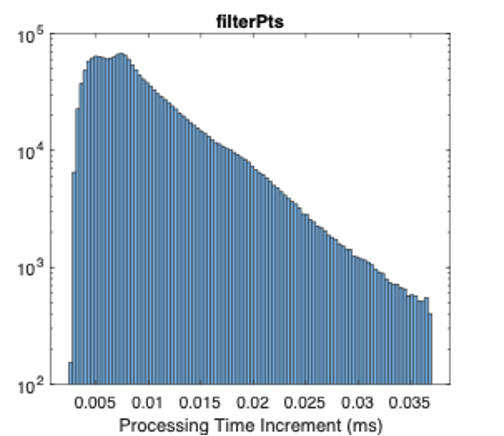
\includegraphics[width=\textwidth]{Images/gbcache/filter_points_hist.png}
        \caption{Histogram of duration of \texttt{filter\_points} against number of LiDAR points}
        \label{fig:gbcache_filter_points_hist}
    \end{subfigure}
}
\caption{Scatter (a) and histogram (b) plots of \texttt{filter\_points} process plotted against number of LiDAR points}
\label{fig:gbcache_filter_points}
\end{figure}

\begin{figure}[htbp]
\centering
\makebox[\textwidth][c]{
    \begin{subfigure}[t]{0.44\textwidth}
        \centering
        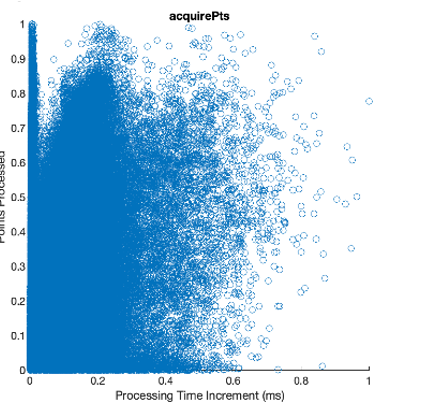
\includegraphics[width=\textwidth]{Images/gbcache/Add_points_scatter.png}
        \caption{Scatter plot of duration of \texttt{add\_points} against number of LiDAR points}
        \label{fig:gbcache_add_points_scatter}
    \end{subfigure}
    \hspace{2em} % horizontal spacing between them
    \begin{subfigure}[t]{0.44\textwidth}
        \centering
        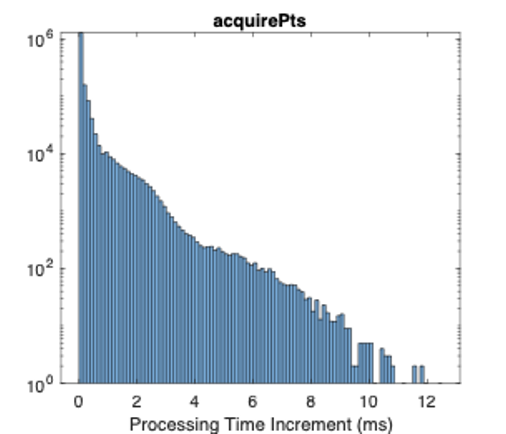
\includegraphics[width=\textwidth]{Images/gbcache/Add_points_hist.png}
        \caption{Histogram of duration of \texttt{add\_points} against number of LiDAR points}
        \label{fig:gbcache_add_points_hist}
    \end{subfigure}
}
\caption{Scatter (a) and histogram (b) plots of \texttt{add\_points} process plotted against number of LiDAR points}
\label{fig:gbcache_add_points}
\end{figure}

\begin{figure}[htbp]
    \centering
    % Subfigure (a)
    \begin{subfigure}[b]{0.44\linewidth}
        \centering
        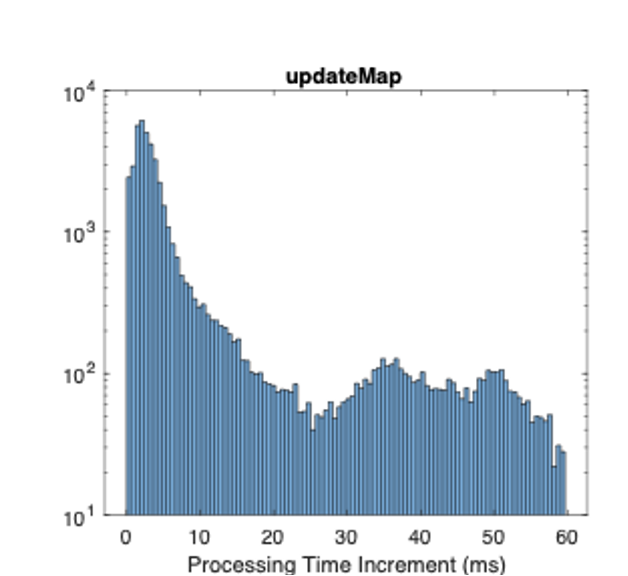
\includegraphics[width=\linewidth]{Images/gbcache/Update_Map_hist.png}
        \caption{Histogram of duration of \texttt{map\_update} against number of LiDAR points}
        \label{fig:gbcache_update_map_hist}
    \end{subfigure}
    \vspace{1em} % vertical spacing between subfigures
    % Subfigure (b)
    \begin{subfigure}[b]{0.8\linewidth}
        \centering
        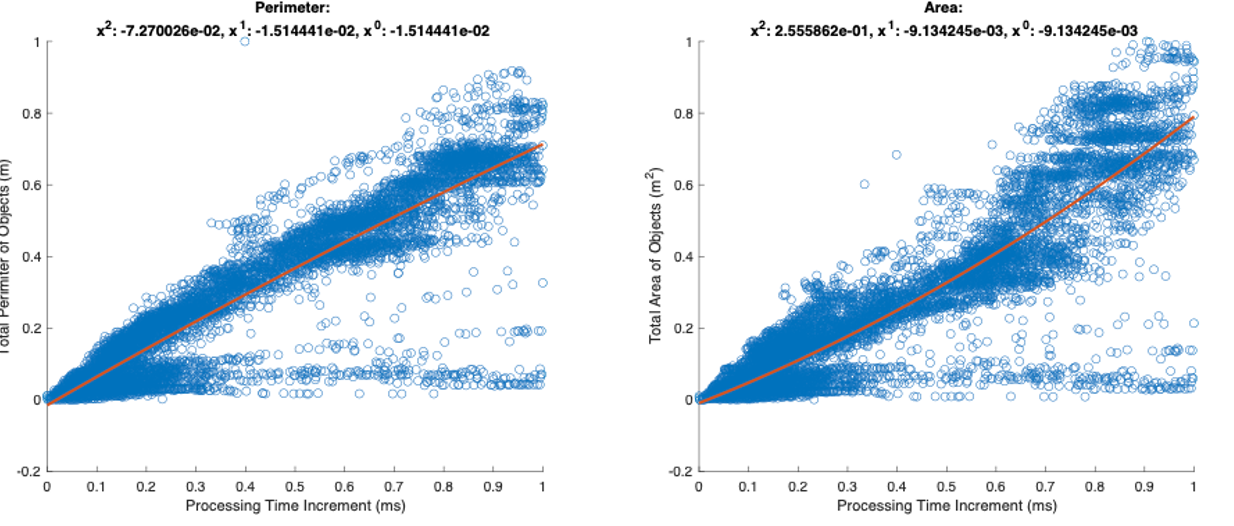
\includegraphics[width=\linewidth]{Images/gbcache/Update_Map_scatter.png}
        \caption{Two scatter plot of duration of \texttt{map\_update} against average perimeter length of polygon (left), and against average area of polygon (right). The line of best-fit is shown in red for each, with associated polynomial values of: $x^2 = -0.0727, x^1 = -0.0151, x^0 = -0.0151$ (left) and $x^2 = 0.2556, x^1 = -0.00913, x^0 = -0.00913$ (right) }
        \label{fig:gbcache_update_map_scatter}
    \end{subfigure}

    \caption{Histogram (a) and scatter (b) plots of \texttt{map\_update} process plotted against number of LiDAR points}
    \label{fig:gbcache_update_map}
\end{figure}

%%%%%%%%%%%%%%%%%%%%%%%%%%%%%%%%%%%%%%%%%%%%%%%%%%%%%%%%%%%%%%%%%%%%
\subsection{Mutual Information Analysis of Features} \label{sec:gbcache_MI_features}

While the ten-feature set provides comprehensive object characterization, not all features contribute equally to classification performance, and some features exhibit redundancy through correlation.
I applied information-theoretic feature selection methodology to identify the optimal feature subset that maximizes classification accuracy while minimizing computational burden and correlation-induced instability.

The minimum Redundancy Maximum Relevance (mRMR) criterion provides a principled framework for feature selection by simultaneously considering two competing objectives: maximizing the mutual information between selected features and class labels (relevance) while minimizing the mutual information among selected features themselves (redundancy).
Mutual information quantifies the reduction in uncertainty about one variable given knowledge of another, providing a model-agnostic measure of statistical dependence applicable to both linear and nonlinear relationships.

Analysis of feature-class mutual information reveals varying discriminative power across the ten features, with intensity-based and geometric features exhibiting complementary strengths for different object classes.
Pairwise feature redundancy analysis identifies multiple correlated feature pairs that provide overlapping information, suggesting opportunities for dimensionality reduction without classification performance degradation.
The mRMR optimization procedure balances these considerations, progressively selecting features that contribute novel discriminative information while avoiding redundant measurements.

Information-theoretic analysis identified an optimal feature subset substantially smaller than the complete ten-feature set, demonstrating that effective maritime object classification can be achieved with reduced feature dimensionality.
This finding has practical implications for computational efficiency, as feature extraction and Gaussian density evaluation scale with feature dimensionality.
The reduced feature set maintains robust classification performance while decreasing processing requirements and reducing the risk of overfitting when training data is limited.

The classifier requires training data comprising labeled examples of each object class with corresponding feature vectors.
Training involves computing maximum likelihood estimates of Gaussian distribution parameters for each class, specifically the mean vector and covariance matrix that characterize the feature space distribution.
These parameters fully specify the class models, enabling rapid inference through simple multivariate Gaussian density evaluation without iterative optimization or complex neural network forward passes.

Classification performance depends critically on the separability of object classes in the chosen feature space and the validity of the Gaussian distribution assumption.
When classes exhibit significant overlap in feature space or when feature distributions deviate substantially from Gaussian, classification accuracy degrades.
However, for maritime objects with distinct geometric profiles and size ranges, the feature-based Gaussian approach provides robust classification with minimal training requirements.

\begin{figure}
    \centering
    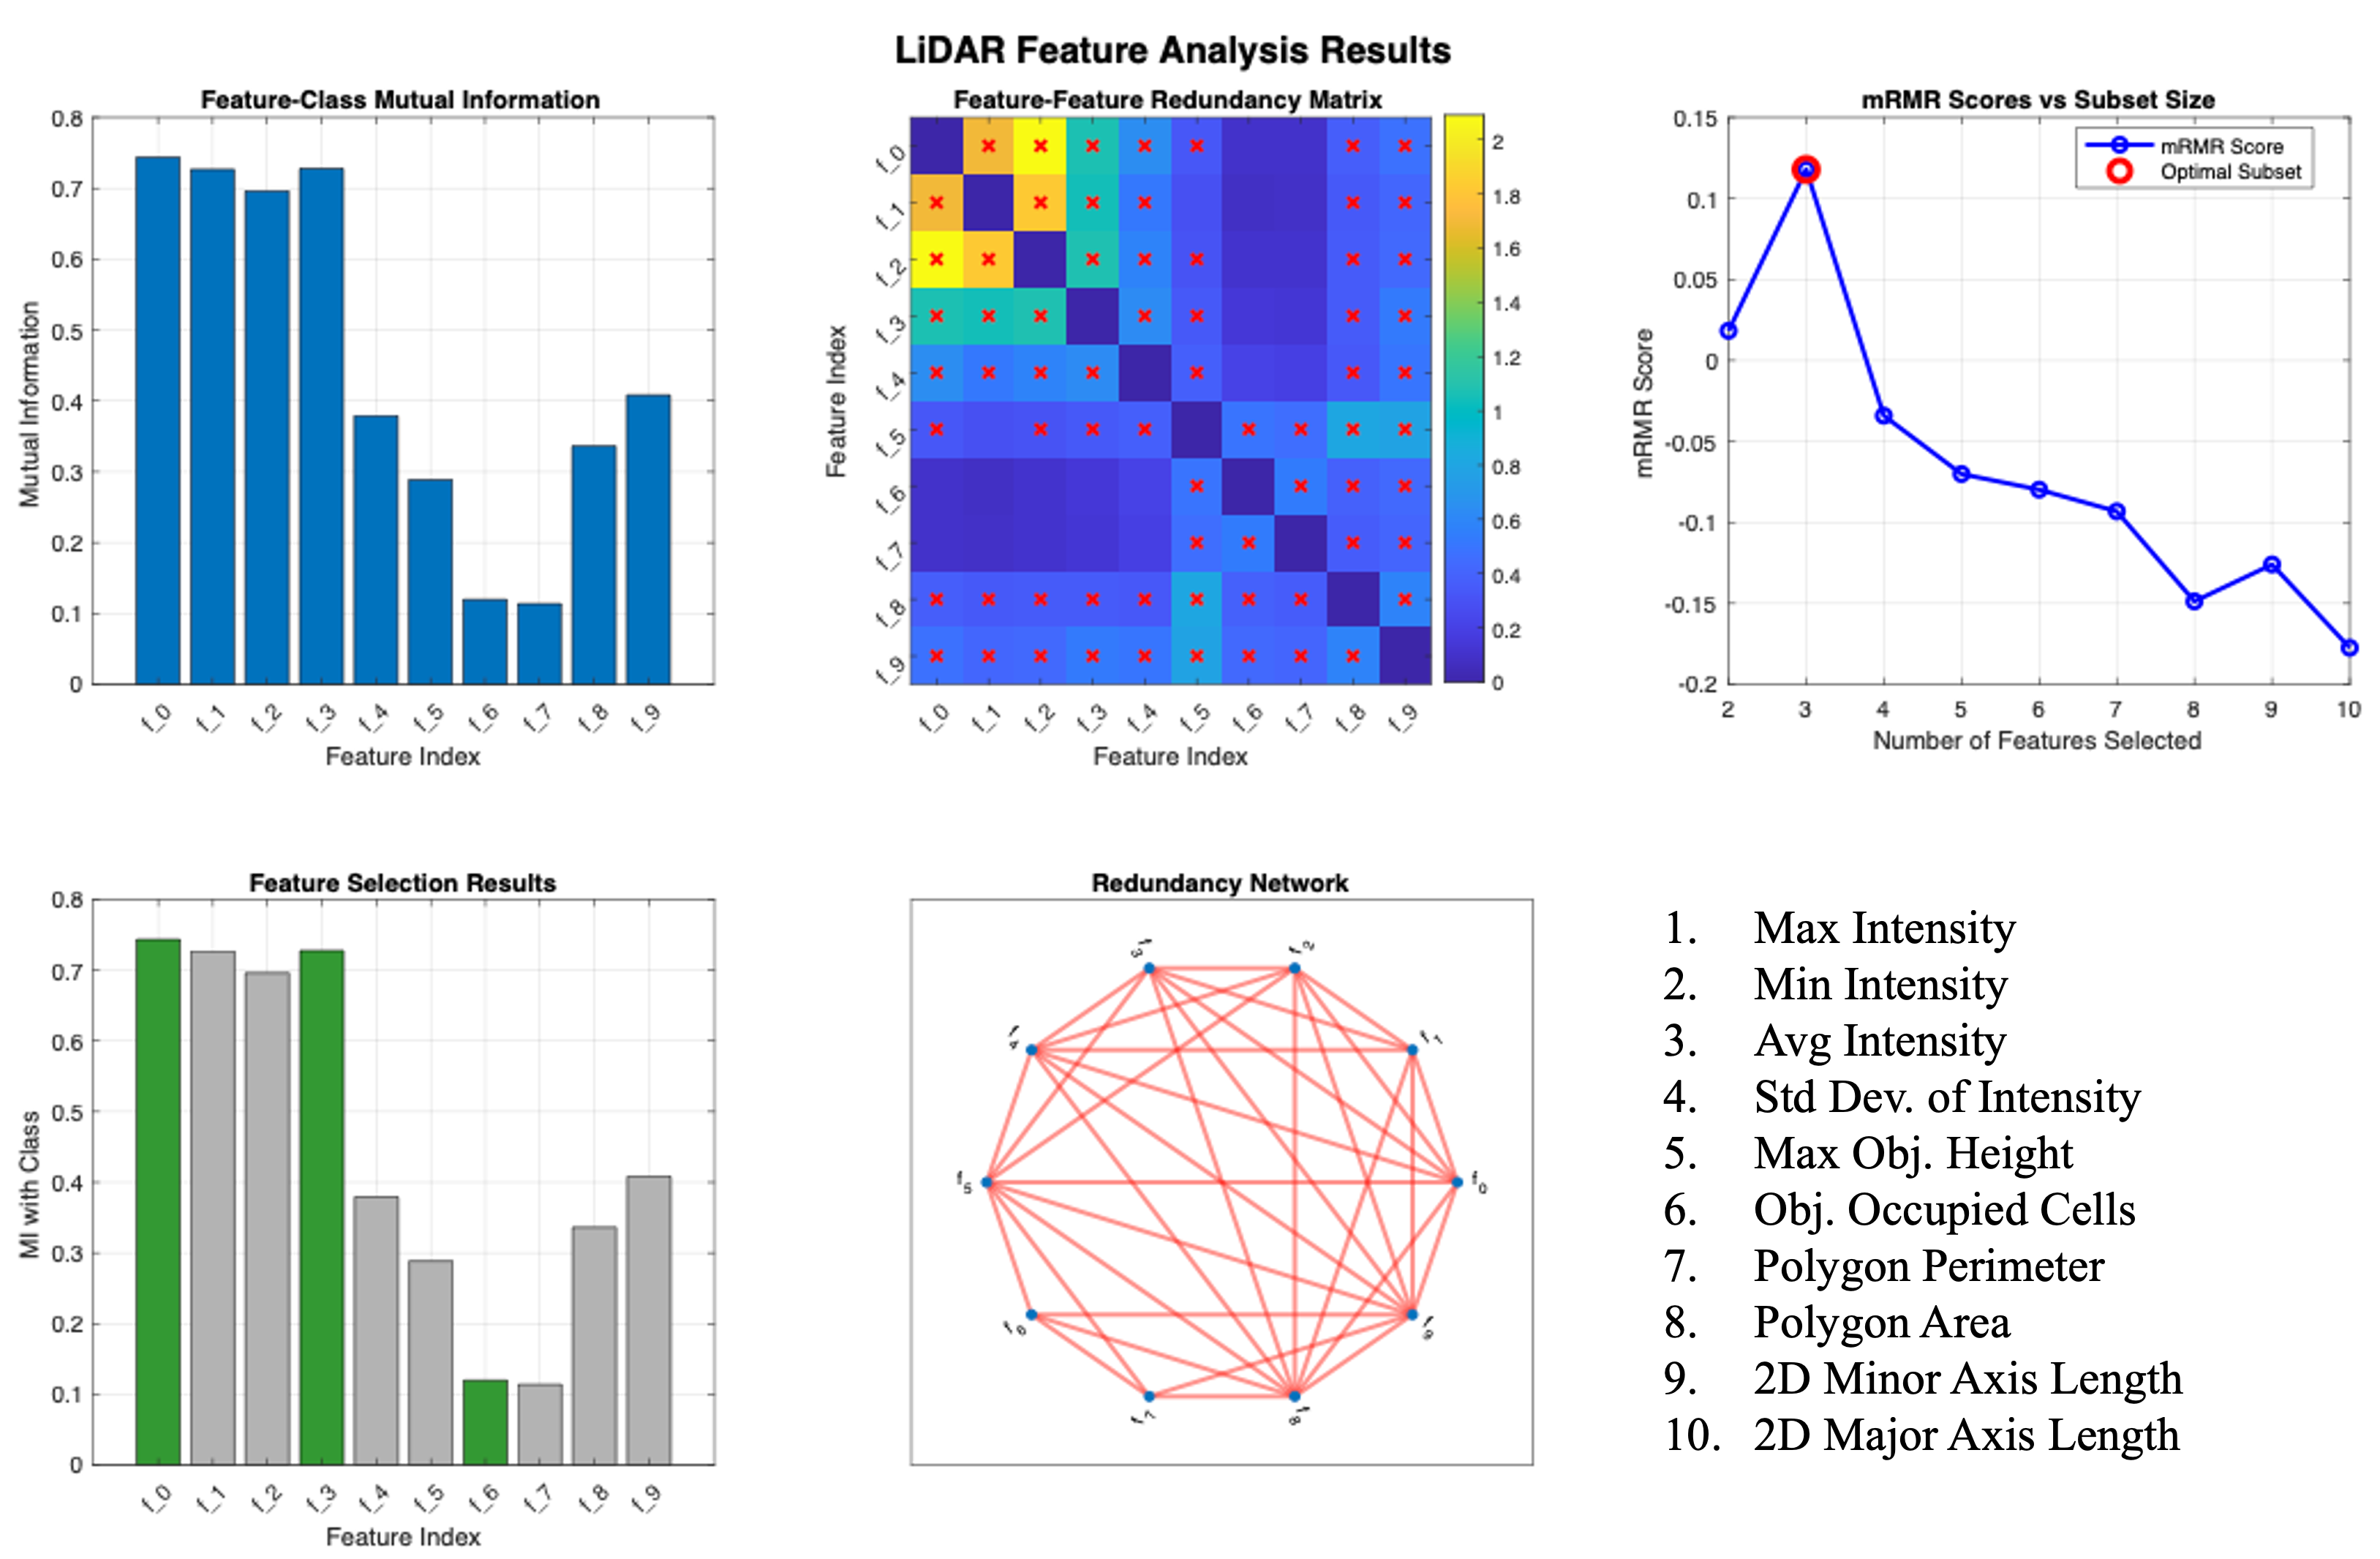
\includegraphics[width=0.95\linewidth]{Images/MI_analysis.png}
    \caption{Caption}
    \label{fig:MI_analysis}
\end{figure}

\begin{figure}
    \centering
    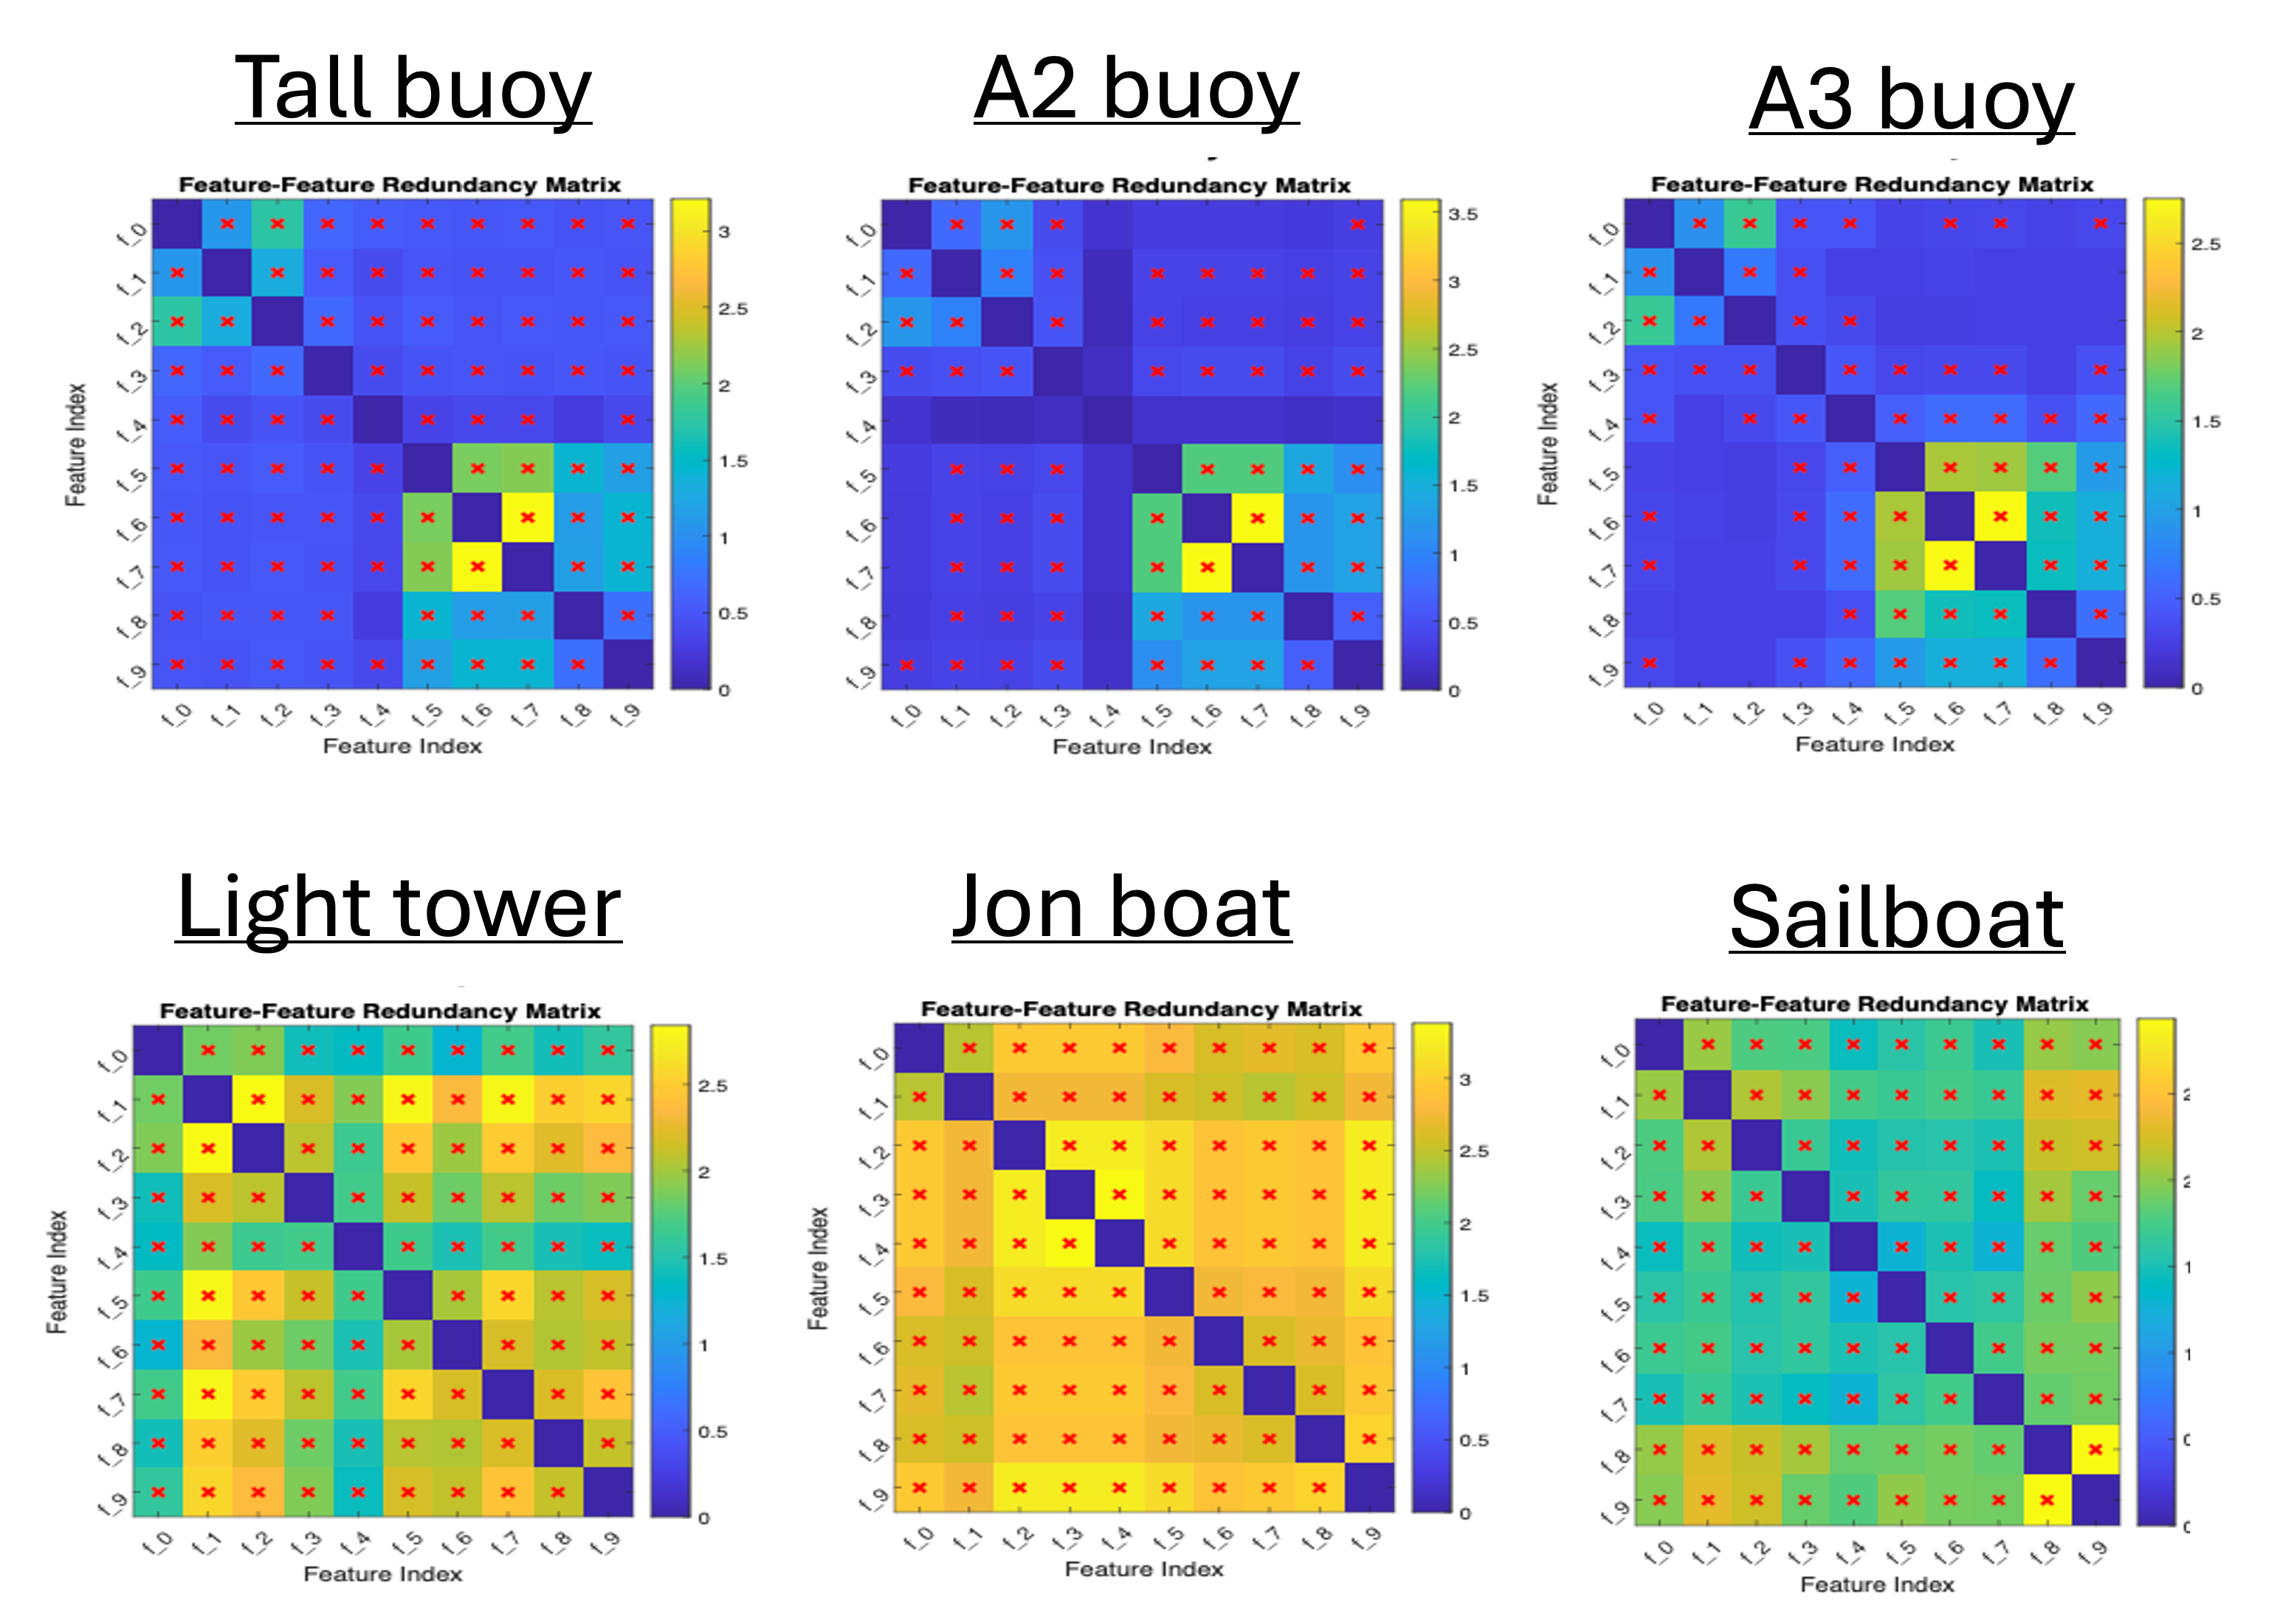
\includegraphics[width=0.95\linewidth]{Images/MI_pairwise.png}
    \caption{Caption}
    \label{fig:MI_pairwise}
\end{figure}

%%%%%%%%%%%%%%%%%%%%%%%%%%%%%%%%%%%%%%%%%%%%%%%%%%%%%%%%%%%%%%%%%%%%
%%%%%%%%%%%%%%%%%%%%%%%%%%%%%%%%%%%%%%%%%%%%%%%%%%%%%%%%%%%%%%%%%%%%
%%%%%%%%%%%%%%%%%%%%%%%%%%%%%%%%%%%%%%%%%%%%%%%%%%%%%%%%%%%%%%%%%%%%


\end{document}
